\documentclass[10pt,landscape]{article}
\usepackage{multicol}
\usepackage{calc}
\usepackage{ifthen}
\usepackage[landscape]{geometry}
\usepackage{hyperref}
\usepackage{graphicx}
\usepackage{tikz}
\usetikzlibrary{positioning,arrows.meta,calc}
\usepackage{lipsum}
\usepackage{adjustbox}


% To make this come out properly in landscape mode, do one of the following
% 1.
%  pdflatex latexsheet.tex
%
% 2.
%  latex latexsheet.tex
%  dvips -P pdf  -t landscape latexsheet.dvi
%  ps2pdf latexsheet.ps


% If you're reading this, be prepared for confusion.  Making this was
% a learning experience for me, and it shows.  Much of the placement
% was hacked in; if you make it better, let me know...


% 2008-04
% Changed page margin code to use the geometry package. Also added code for
% conditional page margins, depending on paper size. Thanks to Uwe Ziegenhagen
% for the suggestions.

% 2006-08
% Made changes based on suggestions from Gene Cooperman. <gene at ccs.neu.edu>


% To Do:
% \listoffigures \listoftables
% \setcounter{secnumdepth}{0}


% This sets page margins to .5 inch if using letter paper, and to 1cm
% if using A4 paper. (This probably isn't strictly necessary.)
% If using another size paper, use default 1cm margins.
\ifthenelse{\lengthtest { \paperwidth = 11in}}
	{ \geometry{top=.5in,left=.5in,right=.5in,bottom=.5in} }
	{\ifthenelse{ \lengthtest{ \paperwidth = 297mm}}
		{\geometry{top=1cm,left=1cm,right=1cm,bottom=1cm} }
		{\geometry{top=1cm,left=1cm,right=1cm,bottom=1cm} }
	}

% Turn off header and footer
\pagestyle{empty}
 

% Redefine section commands to use less space
\makeatletter
\renewcommand{\section}{\@startsection{section}{1}{0mm}%
                                {-1ex plus -.5ex minus -.2ex}%
                                {0.5ex plus .2ex}%x
                                {\normalfont\large\bfseries}}
\renewcommand{\subsection}{\@startsection{subsection}{2}{0mm}%
                                {-1explus -.5ex minus -.2ex}%
                                {0.5ex plus .2ex}%
                                {\normalfont\normalsize\bfseries}}
\renewcommand{\subsubsection}{\@startsection{subsubsection}{3}{0mm}%
                                {-1ex plus -.5ex minus -.2ex}%
                                {1ex plus .2ex}%
                                {\normalfont\small\bfseries}}
\makeatother

% Define BibTeX command
\def\BibTeX{{\rm B\kern-.05em{\sc i\kern-.025em b}\kern-.08em
    T\kern-.1667em\lower.7ex\hbox{E}\kern-.125emX}}

% Don't print section numbers
% \setcounter{secnumdepth}{0}


\setlength{\parindent}{0pt}
\setlength{\parskip}{0pt plus 0.5ex}


% -----------------------------------------------------------------------

\begin{document}

\raggedright
\footnotesize
\begin{multicols}{3}


% multicol parameters
% These lengths are set only within the two main columns
%\setlength{\columnseprule}{0.25pt}
\setlength{\premulticols}{1pt}
\setlength{\postmulticols}{1pt}
\setlength{\multicolsep}{1pt}
\setlength{\columnsep}{2pt}

\begin{center}
     \Large{\textbf{Cheat Sheet}} \\
\end{center}

\section{\LaTeX}
\subsection{Document classes}
\begin{tabular}{@{}ll@{}}
\verb!book!    & Default is two-sided. \\
\verb!report!  & No \verb!\part! divisions. \\
\verb!article! & No \verb!\part! or \verb!\chapter! divisions. \\
\verb!letter!  & Letter (?). \\
\verb!slides!  & Large sans-serif font.
\end{tabular}

Used at the very beginning of a document:
\verb!\documentclass{!\textit{class}\verb!}!.  Use
\verb!\begin{document}! to start contents and \verb!\end{document}! to
end the document.


\subsubsection{Common \texttt{documentclass} options}
\newlength{\MyLen}
\settowidth{\MyLen}{\texttt{letterpaper}/\texttt{a4paper} \ }
\begin{tabular}{@{}p{\the\MyLen}%
                @{}p{\linewidth-\the\MyLen}@{}}
\texttt{10pt}/\texttt{11pt}/\texttt{12pt} & Font size. \\
\texttt{letterpaper}/\texttt{a4paper} & Paper size. \\
\texttt{twocolumn} & Use two columns. \\
\texttt{twoside}   & Set margins for two-sided. \\
\texttt{landscape} & Landscape orientation.  Must use
                     \texttt{dvips -t landscape}. \\
\texttt{draft}     & Double-space lines.
\end{tabular}

Usage:
\verb!\documentclass[!\textit{opt,opt}\verb!]{!\textit{class}\verb!}!.


\subsubsection{Packages}
\settowidth{\MyLen}{\texttt{multicol} }
\begin{tabular}{@{}p{\the\MyLen}%
                @{}p{\linewidth-\the\MyLen}@{}}
%\begin{tabular}{@{}ll@{}}
\texttt{fullpage}  &  Use 1 inch margins. \\
\texttt{anysize}   &  Set margins: \verb!\marginsize{!\textit{l}%
                        \verb!}{!\textit{r}\verb!}{!\textit{t}%
                        \verb!}{!\textit{b}\verb!}!.            \\
\texttt{multicol}  &  Use $n$ columns: 
                        \verb!\begin{multicols}{!$n$\verb!}!.   \\
\texttt{latexsym}  &  Use \LaTeX\ symbol font. \\
\texttt{graphicx}  &  Show image:
                        \verb!\includegraphics[width=!%
                        \textit{x}\verb!]{!%
                        \textit{file}\verb!}!. \\
\texttt{url}       & Insert URL: \verb!\url{!%
                        \textit{http://\ldots}%
                        \verb!}!.
\end{tabular}

Use before \verb!\begin{document}!. 
Usage: \verb!\usepackage{!\textit{package}\verb!}!


\subsubsection{Title}
\settowidth{\MyLen}{\texttt{.author.text.} }
\begin{tabular}{@{}p{\the\MyLen}%
                @{}p{\linewidth-\the\MyLen}@{}}
\verb!\author{!\textit{text}\verb!}! & Author of document. \\
\verb!\title{!\textit{text}\verb!}!  & Title of document. \\
\verb!\date{!\textit{text}\verb!}!   & Date. \\
\end{tabular}

These commands go before \verb!\begin{document}!.  The declaration
\verb!\maketitle! goes at the top of the document.

\subsubsection{Miscellaneous}
\settowidth{\MyLen}{\texttt{.pagestyle.empty.} }
\begin{tabular}{@{}p{\the\MyLen}%
                @{}p{\linewidth-\the\MyLen}@{}}
\verb!\pagestyle{empty}!     &   Empty header, footer
                                 and no page numbers. \\
\verb!\tableofcontents!      &   Add a table of contents here. \\

\end{tabular}



\subsection{Document structure}
\begin{multicols}{2}
\verb!\part{!\textit{title}\verb!}!  \\
\verb!\chapter{!\textit{title}\verb!}!  \\
\verb!\subsection{!\textit{title}\verb!}!  \\
\verb!\subsubsection{!\textit{title}\verb!}!  \\
\verb!\paragraph{!\textit{title}\verb!}!  \\
\verb!\paragraph{!\textit{title}\verb!}!  \\
\verb!\subparagraph{!\textit{title}\verb!}!
\end{multicols}
{\raggedright
Use \verb!\setcounter{secnumdepth}{!$x$\verb!}! suppresses heading
numbers of depth $>x$, where \verb!chapter! has depth 0.
Use a \texttt{*}, as in \verb!\subsection*{!\textit{title}\verb!}!,
to not number a particular item---these items will also not appear
in the table of contents.
}

\subsubsection{Text environments}
\settowidth{\MyLen}{\texttt{.begin.quotation.}}
\begin{tabular}{@{}p{\the\MyLen}%
                @{}p{\linewidth-\the\MyLen}@{}}
\verb!\begin{comment}!    &  Comment (not printed). Requires \texttt{verbatim} package. \\
\verb!\begin{quote}!      &  Indented quotation block. \\
\verb!\begin{quotation}!  &  Like \texttt{quote} with indented paragraphs. \\
\verb!\begin{verse}!      &  Quotation block for verse.
\end{tabular}

\subsubsection{Lists}
\settowidth{\MyLen}{\texttt{.begin.description.}}
\begin{tabular}{@{}p{\the\MyLen}%
                @{}p{\linewidth-\the\MyLen}@{}}
\verb!\begin{enumerate}!        &  Numbered list. \\
\verb!\begin{itemize}!          &  Bulleted list. \\
\verb!\begin{description}!      &  Description list. \\
\verb!\item! \textit{text}      &  Add an item. \\
\verb!\item[!\textit{x}\verb!]! \textit{text}
                                &  Use \textit{x} instead of normal
                        bullet or number.  Required for descriptions. \\
\end{tabular}




\subsubsection{References}
\settowidth{\MyLen}{\texttt{.pageref.marker..}}
\begin{tabular}{@{}p{\the\MyLen}%
                @{}p{\linewidth-\the\MyLen}@{}}
\verb!\label{!\textit{marker}\verb!}!   &  Set a marker for cross-reference, 
                          often of the form \verb!\label{sec:item}!. \\
\verb!\ref{!\textit{marker}\verb!}!   &  Give subsection/body number of marker. \\
\verb!\pageref{!\textit{marker}\verb!}! &  Give page number of marker. \\
\verb!\footnote{!\textit{text}\verb!}!  &  Print footnote at bottom of page. \\
\end{tabular}
\begin{verbatim}
\usepackage{hyperref}
  [...]
\hyperlink{marker}{clickable link text}
\end{verbatim}


\subsubsection{Floating bodies}
\settowidth{\MyLen}{\texttt{.begin.equation..place.}}
\begin{tabular}{@{}p{\the\MyLen}%
                @{}p{\linewidth-\the\MyLen}@{}}
\verb!\begin{table}[!\textit{place}\verb!]!     &  Add numbered table. \\
\verb!\begin{figure}[!\textit{place}\verb!]!    &  Add numbered figure. \\
\verb!\begin{equation}[!\textit{place}\verb!]!  &  Add numbered equation. \\
\verb!\caption{!\textit{text}\verb!}!           &  Caption for the body. \\
\end{tabular}

The \textit{place} is a list valid placements for the body.  \texttt{t}=top,
\texttt{h}=here, \texttt{b}=bottom, \texttt{p}=separate page, \texttt{!}=place even if ugly.  Captions and label markers should be within the environment.

%---------------------------------------------------------------------------

\subsection{Text properties}

\subsubsection{Font face}
\newcommand{\FontCmd}[3]{\PBS\verb!\#1{!\textit{text}\verb!}!  \> %
                         \verb!{\#2 !\textit{text}\verb!}! \> %
                         \#1{#3}}
\begin{tabular}{@{}l@{}l@{}l@{}}
\textit{Command} & \textit{Declaration} & \textit{Effect} \\
\verb!\textrm{!\textit{text}\verb!}!                    & %
        \verb!{\rmfamily !\textit{text}\verb!}!               & %
        \textrm{Roman family} \\
\verb!\textsf{!\textit{text}\verb!}!                    & %
        \verb!{\sffamily !\textit{text}\verb!}!               & %
        \textsf{Sans serif family} \\
\verb!\texttt{!\textit{text}\verb!}!                    & %
        \verb!{\ttfamily !\textit{text}\verb!}!               & %
        \texttt{Typewriter family} \\
\verb!\textmd{!\textit{text}\verb!}!                    & %
        \verb!{\mdseries !\textit{text}\verb!}!               & %
        \textmd{Medium series} \\
\verb!\textbf{!\textit{text}\verb!}!                    & %
        \verb!{\bfseries !\textit{text}\verb!}!               & %
        \textbf{Bold series} \\
\verb!\textup{!\textit{text}\verb!}!                    & %
        \verb!{\upshape !\textit{text}\verb!}!               & %
        \textup{Upright shape} \\
\verb!\textit{!\textit{text}\verb!}!                    & %
        \verb!{\itshape !\textit{text}\verb!}!               & %
        \textit{Italic shape} \\
\verb!\textsl{!\textit{text}\verb!}!                    & %
        \verb!{\slshape !\textit{text}\verb!}!               & %
        \textsl{Slanted shape} \\
\verb!\textsc{!\textit{text}\verb!}!                    & %
        \verb!{\scshape !\textit{text}\verb!}!               & %
        \textsc{Small Caps shape} \\
\verb!\emph{!\textit{text}\verb!}!                      & %
        \verb!{\em !\textit{text}\verb!}!               & %
        \emph{Emphasized} \\
\verb!\textnormal{!\textit{text}\verb!}!                & %
        \verb!{\normalfont !\textit{text}\verb!}!       & %
        \textnormal{Document font} \\
\verb!\underline{!\textit{text}\verb!}!                 & %
                                                        & %
        \underline{Underline}
\end{tabular}

The command (t\textit{tt}t) form handles spacing better than the
declaration (t{\itshape tt}t) form.

\subsubsection{Font size}
\setlength{\columnsep}{14pt} % Need to move columns apart a little
\begin{multicols}{2}
\begin{tabbing}
\verb!\footnotesize!          \= \kill
\verb!\tiny!                  \>  \tiny{tiny} \\
\verb!\scriptsize!            \>  \scriptsize{scriptsize} \\
\verb!\footnotesize!          \>  \footnotesize{footnotesize} \\
\verb!\small!                 \>  \small{small} \\
\verb!\normalsize!            \>  \normalsize{normalsize} \\
\verb!\large!                 \>  \large{large} \\
\verb!\Large!                 \=  \Large{Large} \\  % Tab hack for new column
\verb!\LARGE!                 \>  \LARGE{LARGE} \\
\verb!\huge!                  \>  \huge{huge} \\
\verb!\Huge!                  \>  \Huge{Huge}
\end{tabbing}
\end{multicols}
\setlength{\columnsep}{1pt} % Set column separation back

These are declarations and should be used in the form
\verb!{\small! \ldots\verb!}!, or without braces to affect the entire
document.

Specifying an arbitrary fontsize:
\begin{verbatim}
\usepackage{scalefnt}
[...]
\begingroup
\scalefont{2.0} 2 times the original font size
\endgroup
\end{verbatim}
\begingroup
\scalefont{2.0} 2 times the original font size
\endgroup



\subsubsection{Verbatim text}

\settowidth{\MyLen}{\texttt{.begin.verbatim..} }
\begin{tabular}{@{}p{\the\MyLen}%
                @{}p{\linewidth-\the\MyLen}@{}}
\verb@\begin{verbatim}@ & Verbatim environment. \\
\verb@\begin{verbatim*}@ & Spaces are shown as \verb*@ @. \\
\verb@\verb!text!@ & Text between the delimiting characters (in this case %
                      `\texttt{!}') is verbatim.
\end{tabular}


\subsubsection{Justification}
\begin{tabular}{@{}ll@{}}
\textit{Environment}  &  \textit{Declaration}  \\
\verb!\begin{center}!      & \verb!\centering!  \\
\verb!\begin{flushleft}!  & \verb!\raggedright! \\
\verb!\begin{flushright}! & \verb!\raggedleft!  \\
\end{tabular}

\subsubsection{Miscellaneous}
\verb!\linespread{!$x$\verb!}! changes the line spacing by the
multiplier $x$.





\subsection{Text-mode symbols}

\subsubsection{Symbols}
\begin{tabular}{@{}l@{\hspace{1em}}l@{\hspace{2em}}l@{\hspace{1em}}l@{\hspace{2em}}l@{\hspace{1em}}l@{\hspace{2em}}l@{\hspace{1em}}l@{}}
\&              &  \verb!\&! &
\_              &  \verb!\_! &
\ldots          &  \verb!\ldots! &
\textbullet     &  \verb!\textbullet! \\
\$              &  \verb!\$! &
\^{}            &  \verb!\^{}! &
\textbar        &  \verb!\textbar! &
\textbackslash  &  \verb!\textbackslash! \\
\%              &  \verb!\%! &
\~{}            &  \verb!\~{}! &
\#              &  \verb!\#! &
\S              &  \verb!\S! \\
\end{tabular}

\subsubsection{Accents}
\begin{tabular}{@{}l@{\ }l|l@{\ }l|l@{\ }l|l@{\ }l|l@{\ }l@{}}
\`o   & \verb!\`o! &
\'o   & \verb!\'o! &
\^o   & \verb!\^o! &
\~o   & \verb!\~o! &
\=o   & \verb!\=o! \\
\.o   & \verb!\.o! &
\"o   & \verb!\"o! &
\c o  & \verb!\c o! &
\v o  & \verb!\v o! &
\H o  & \verb!\H o! \\
\c c  & \verb!\c c! &
\d o  & \verb!\d o! &
\b o  & \verb!\b o! &
\t oo & \verb!\t oo! &
\oe   & \verb!\oe! \\
\OE   & \verb!\OE! &
\ae   & \verb!\ae! &
\AE   & \verb!\AE! &
\aa   & \verb!\aa! &
\AA   & \verb!\AA! \\
\o    & \verb!\o! &
\O    & \verb!\O! &
\l    & \verb!\l! &
\L    & \verb!\L! &
\i    & \verb!\i! \\
\j    & \verb!\j! &
!`    & \verb!~`! &
?`    & \verb!?`! &
\end{tabular}


\subsubsection{Delimiters}
\begin{tabular}{@{}l@{\ }ll@{\ }ll@{\ }ll@{\ }ll@{\ }ll@{\ }l@{}}
`       & \verb!`!  &
``      & \verb!``! &
\{      & \verb!\{! &
\lbrack & \verb![! &
(       & \verb!(! &
\textless  &  \verb!\textless! \\
'       & \verb!'!  &
''      & \verb!''! &
\}      & \verb!\}! &
\rbrack & \verb!]! &
)       & \verb!)! &
\textgreater  &  \verb!\textgreater! \\
\end{tabular}

\subsubsection{Dashes}
\begin{tabular}{@{}llll@{}}
\textit{Name} & \textit{Source} & \textit{Example} & \textit{Usage} \\
hyphen  & \verb!-!   & X-ray          & In words. \\
en-dash & \verb!--!  & 1--5           & Between numbers. \\
em-dash & \verb!---! & Yes---or no?    & Punctuation.
\end{tabular}


\subsubsection{Line and page breaks}
\settowidth{\MyLen}{\texttt{.pagebreak} }
\begin{tabular}{@{}p{\the\MyLen}%
                @{}p{\linewidth-\the\MyLen}@{}}
\verb!\\!          &  Begin new line without new paragraph.  \\
\verb!\\*!         &  Prohibit pagebreak after linebreak. \\
\verb!\kill!       &  Don't print current line. \\
\verb!\pagebreak!  &  Start new page. \\
\verb!\noindent!   &  Do not indent current line.
\end{tabular}


\subsubsection{Miscellaneous}
\settowidth{\MyLen}{\texttt{.rule.w..h.} }
\begin{tabular}{@{}p{\the\MyLen}%
                @{}p{\linewidth-\the\MyLen}@{}}
\verb!\today!  &  \today. \\
\verb!$\sim$!  &  Prints $\sim$ instead of \verb!\~{}!, which makes \~{}. \\
\verb!~!       &  Space, disallow linebreak (\verb!W.J.~Clinton!). \\
\verb!\@.!     &  Indicate that the \verb!.! ends a sentence when following
                        an uppercase letter. \\
\verb!\hspace{!$l$\verb!}! & Horizontal space of length $l$
                                (Ex: $l=\mathtt{20pt}$). \\
\verb!\vspace{!$l$\verb!}! & Vertical space of length $l$. \\
\verb!\rule{!$w$\verb!}{!$h$\verb!}! & Line of width $w$ and height $h$. \\
\end{tabular}



\subsection{Tabular environments}

\subsubsection{\texttt{tabbing} environment}
\begin{tabular}{@{}l@{\hspace{1.5ex}}l@{\hspace{10ex}}l@{\hspace{1.5ex}}l@{}}
\verb!\=!  &   Set tab stop. &
\verb!\>!  &   Go to tab stop.
\end{tabular}

Tab stops can be set on ``invisible'' lines with \verb!\kill!
at the end of the line.  Normally \verb!\\! is used to separate lines.


\subsubsection{\texttt{tabular} environment}
\verb!\begin{array}[!\textit{pos}\verb!]{!\textit{cols}\verb!}!   \\
\verb!\begin{tabular}[!\textit{pos}\verb!]{!\textit{cols}\verb!}! \\
\verb!\begin{tabular*}{!\textit{width}\verb!}[!\textit{pos}\verb!]{!\textit{cols}\verb!}!


\paragraph{\texttt{tabular} column specification}
\settowidth{\MyLen}{\texttt{p}\{\textit{width}\} \ }
\begin{tabular}{@{}p{\the\MyLen}@{}p{\linewidth-\the\MyLen}@{}}
\texttt{l}    &   Left-justified column.  \\
\texttt{c}    &   Centered column.  \\
\texttt{r}    &   Right-justified column. \\
\verb!p{!\textit{width}\verb!}!  &  Same as %
                              \verb!\parbox[t]{!\textit{width}\verb!}!. \\ 
\verb!@{!\textit{decl}\verb!}!   &  Insert \textit{decl} instead of
                                    inter-column space. \\
\verb!|!      &   Inserts a vertical line between columns. 
\end{tabular}


\paragraph{\texttt{tabular} elements}
\settowidth{\MyLen}{\texttt{.cline.x-y..}}
\begin{tabular}{@{}p{\the\MyLen}@{}p{\linewidth-\the\MyLen}@{}}
\verb!\hline!           &  Horizontal line between rows.  \\
\verb!\cline{!$x$\verb!-!$y$\verb!}!  &
                        Horizontal line across columns $x$ through $y$. \\
\verb!\multicolumn{!\textit{n}\verb!}{!\textit{cols}\verb!}{!\textit{text}\verb!}! \\
        &  A cell that spans \textit{n} columns, with \textit{cols} column specification.
\end{tabular}

\subsection{Math mode}
For inline math, use \verb!\(...\)! or \verb!$...$!.
For displayed math, use \verb!\[...\]! or \verb!\begin{equation}!.

\begin{tabular}{@{}l@{\hspace{1em}}l@{\hspace{2em}}l@{\hspace{1em}}l@{}}
Superscript$^{x}$       &
\verb!^{x}!             &  
Subscript$_{x}$         &
\verb!_{x}!             \\  
$\frac{x}{y}$           &
\verb!\frac{x}{y}!      &  
$\sum_{k=1}^n$          &
\verb!\sum_{k=1}^n!     \\  
$\sqrt[n]{x}$           &
\verb!\sqrt[n]{x}!      &  
$\prod_{k=1}^n$         &
\verb!\prod_{k=1}^n!    \\ 
\end{tabular}

\subsubsection{Math-mode symbols}

% The ordering of these symbols is slightly odd.  This is because I had to put all the
% long pieces of text in the same column (the right) for it all to fit properly.
% Otherwise, it wouldn't be possible to fit four columns of symbols here.

\begin{tabular}{@{}l@{\hspace{1ex}}l@{\hspace{1em}}l@{\hspace{1ex}}l@{\hspace{1em}}l@{\hspace{1ex}} l@{\hspace{1em}}l@{\hspace{1ex}}l@{}}
$\leq$          &  \verb!\leq!  &
$\geq$          &  \verb!\geq!  &
$\neq$          &  \verb!\neq!  &
$\approx$       &  \verb!\approx!  \\
$\times$        &  \verb!\times!  &
$\div$          &  \verb!\div!  &
$\pm$           & \verb!\pm!  &
$\cdot$         &  \verb!\cdot!  \\
$^{\circ}$      & \verb!^{\circ}! &
$\circ$         &  \verb!\circ!  &
$\prime$        & \verb!\prime!  &
$\cdots$        &  \verb!\cdots!  \\
$\infty$        & \verb!\infty!  &
$\neg$          & \verb!\neg!  &
$\wedge$        & \verb!\wedge!  &
$\vee$          & \verb!\vee!  \\
$\supset$       & \verb!\supset!  &
$\forall$       & \verb!\forall!  &
$\in$           & \verb!\in!  &
$\rightarrow$   &  \verb!\rightarrow! \\
$\subset$       & \verb!\subset!  &
$\exists$       & \verb!\exists!  &
$\notin$        & \verb!\notin!  &
$\Rightarrow$   &  \verb!\Rightarrow! \\
$\cup$          & \verb!\cup!  &
$\cap$          & \verb!\cap!  &
$\mid$          & \verb!\mid!  &
$\Leftrightarrow$   &  \verb!\Leftrightarrow! \\
$\dot a$        & \verb!\dot a!  &
$\hat a$        & \verb!\hat a!  &
$\bar a$        & \verb!\bar a!  &
$\tilde a$      & \verb!\tilde a!  \\

$\alpha$        &  \verb!\alpha!  &
$\beta$         &  \verb!\beta!  &
$\gamma$        &  \verb!\gamma!  &
$\delta$        &  \verb!\delta!  \\
$\epsilon$      &  \verb!\epsilon!  &
$\zeta$         &  \verb!\zeta!  &
$\eta$          &  \verb!\eta!  &
$\varepsilon$   &  \verb!\varepsilon!  \\
$\theta$        &  \verb!\theta!  &
$\iota$         &  \verb!\iota!  &
$\kappa$        &  \verb!\kappa!  &
$\vartheta$     &  \verb!\vartheta!  \\
$\lambda$       &  \verb!\lambda!  &
$\mu$           &  \verb!\mu!  &
$\nu$           &  \verb!\nu!  &
$\xi$           &  \verb!\xi!  \\
$\pi$           &  \verb!\pi!  &
$\rho$          &  \verb!\rho!  &
$\sigma$        &  \verb!\sigma!  &
$\tau$          &  \verb!\tau!  \\
$\upsilon$      &  \verb!\upsilon!  &
$\phi$          &  \verb!\phi!  &
$\chi$          &  \verb!\chi!  &
$\psi$          &  \verb!\psi!  \\
$\omega$        &  \verb!\omega!  &
$\Gamma$        &  \verb!\Gamma!  &
$\Delta$        &  \verb!\Delta!  &
$\Theta$        &  \verb!\Theta!  \\
$\Lambda$       &  \verb!\Lambda!  &
$\Xi$           &  \verb!\Xi!  &
$\Pi$           &  \verb!\Pi!  &
$\Sigma$        &  \verb!\Sigma!  \\
$\Upsilon$      &  \verb!\Upsilon!  &
$\Phi$          &  \verb!\Phi!  &
$\Psi$          &  \verb!\Psi!  &
$\Omega$        &  \verb!\Omega!  
\end{tabular}
\footnotesize

%\subsubsection{Special symbols}
%\begin{tabular}{@{}ll@{}}
%$^{\circ}$  &  \verb!^{\circ}! Ex: $22^{\circ}\mathrm{C}$: \verb!$22^{\circ}\mathrm{C}$!.
%\end{tabular}

\subsection{Bibliography and citations}
When using \BibTeX, you need to run \texttt{latex}, \texttt{bibtex},
and \texttt{latex} twice more to resolve dependencies.

\subsubsection{Citation types}
\settowidth{\MyLen}{\texttt{.shortciteN.key..}}
\begin{tabular}{@{}p{\the\MyLen}@{}p{\linewidth-\the\MyLen}@{}}
\verb!\cite{!\textit{key}\verb!}!       &
        Full author list and year. (Watson and Crick 1953) \\
\verb!\citeA{!\textit{key}\verb!}!      &
        Full author list. (Watson and Crick) \\
\verb!\citeN{!\textit{key}\verb!}!      &
        Full author list and year. Watson and Crick (1953) \\
\verb!\shortcite{!\textit{key}\verb!}!  &
        Abbreviated author list and year. ? \\
\verb!\shortciteA{!\textit{key}\verb!}! &
        Abbreviated author list. ? \\
\verb!\shortciteN{!\textit{key}\verb!}! &
        Abbreviated author list and year. ? \\
\verb!\citeyear{!\textit{key}\verb!}!   &
        Cite year only. (1953) \\
\end{tabular}

All the above have an \texttt{NP} variant without parentheses;
Ex. \verb!\citeNP!.


\subsubsection{\BibTeX\ entry types}
\settowidth{\MyLen}{\texttt{.mastersthesis.}}
\begin{tabular}{@{}p{\the\MyLen}@{}p{\linewidth-\the\MyLen}@{}}
\verb!@article!         &  Journal or magazine article. \\
\verb!@book!            &  Book with publisher. \\
\verb!@booklet!         &  Book without publisher. \\
\verb!@conference!      &  Article in conference proceedings. \\
\verb!@inbook!          &  A part of a book and/or range of pages. \\
\verb!@incollection!    &  A part of book with its own title. \\
%\verb!@manual!          &  Technical documentation. \\
%\verb!@mastersthesis!   &  Master's thesis. \\
\verb!@misc!            &  If nothing else fits. \\
\verb!@phdthesis!       &  PhD. thesis. \\
\verb!@proceedings!     &  Proceedings of a conference. \\
\verb!@techreport!      &  Tech report, usually numbered in series. \\
\verb!@unpublished!     &  Unpublished. \\
\end{tabular}

\subsubsection{\BibTeX\ fields}
\settowidth{\MyLen}{\texttt{organization.}}
\begin{tabular}{@{}p{\the\MyLen}@{}p{\linewidth-\the\MyLen}@{}}
\verb!address!         &  Address of publisher.  Not necessary for major
                                publishers.  \\
\verb!author!           &  Names of authors, of format .... \\
\verb!booktitle!        &  Title of book when part of it is cited. \\
\verb!chapter!          &  Chapter or subsection number. \\
\verb!edition!          &  Edition of a book. \\
\verb!editor!           &  Names of editors. \\
\verb!institution!      &  Sponsoring institution of tech.\ report. \\
\verb!journal!          &  Journal name. \\
\verb!key!              &  Used for cross ref.\ when no author. \\
\verb!month!            &  Month published. Use 3-letter abbreviation. \\
\verb!note!             &  Any additional information. \\
\verb!number!           &  Number of journal or magazine. \\
\verb!organization!     &  Organization that sponsors a conference. \\
\verb!pages!            &  Page range (\verb!2,6,9--12!). \\
\verb!publisher!        &  Publisher's name. \\
\verb!school!           &  Name of school (for thesis). \\
\verb!series!           &  Name of series of books. \\
\verb!title!            &  Title of work. \\
\verb!type!             &  Type of tech.\ report, ex. ``Research Note''. \\
\verb!volume!           &  Volume of a journal or book. \\
\verb!year!             &  Year of publication. \\
\end{tabular}
Not all fields need to be filled.  See example below.

\subsubsection{Common \BibTeX\ style files}
\begin{tabular}{@{}l@{\hspace{1em}}l@{\hspace{3em}}l@{\hspace{1em}}l@{}}
\verb!abbrv!    &  Standard &
\verb!abstract! &  \texttt{alpha} with abstract \\
\verb!alpha!    &  Standard &
\verb!apa!      &  APA \\
\verb!plain!    &  Standard &
\verb!unsrt!    &  Unsorted \\
\end{tabular}

The \LaTeX\ document should have the following two lines just before
\verb!\end{document}!, where \verb!bibfile.bib! is the name of the
\BibTeX\ file.
\begin{verbatim}
\bibliographystyle{plain}
\bibliography{bibfile}
\end{verbatim}

\subsubsection{\BibTeX\ example}
The \BibTeX\ database goes in a file called
\textit{file}\texttt{.bib}, which is processed with \verb!bibtex file!. 
\begin{verbatim}
@String{N = {Na\-ture}}
@Article{WC:1953,
  author  = {James Watson and Francis Crick},
  title   = {A structure for Deoxyribose Nucleic Acid},
  journal = N,
  volume  = {171},
  pages   = {737},
  year    = 1953
}
\end{verbatim}


\subsection{Sample \LaTeX\ document}
\begin{verbatim}
\documentclass[11pt]{article}
\usepackage{fullpage}
\title{Template}
\author{Name}
\begin{document}
\maketitle

\subsection{subsection}
\subsubsection*{subsubsection without number}
text \textbf{bold text} text. Some math: $2+2=5$
\subsubsection{subsubsection}
text \emph{emphasized text} text. \cite{WC:1953}
discovered the structure of DNA.

A table:
\begin{table}[!th]
\begin{tabular}{|l|c|r|}
\hline
first  &  row  &  data \\
second &  row  &  data \\
\hline
\end{tabular}
\caption{This is the caption}
\label{ex:table}
\end{table}

The table is numbered \ref{ex:table}.
\end{document}
\end{verbatim}



\rule{0.3\linewidth}{0.25pt}
\scriptsize

Copyright \copyright\ 2014 Winston Chang

\href{http://wch.github.io/latexsheet/}{http://wch.github.io/latexsheet/}



\newpage
\subsection{adjustbox: adjust boxed content}
\begin{verbatim}
\usepackage{adjustbox}
...
\begin{adjustbox}{
  max totalsize={\textwidth}{\textheight},center}
\end{adjustbox}
\end{verbatim}

\subsection{minipage}
\begin{minipage}[c]{3cm}
  \lipsum[][1-3]
\end{minipage}
\begin{minipage}[c]{3cm}
  \begin{verbatim}
\begin{minipage}[c]{3cm}
  \lipsum[][1-3]
\end{minipage}
  \end{verbatim}
\end{minipage}

\subsection{Beamer class}

\subsubsection{Accessing section names}
\verb |\secname|\\
\verb |\subsecname|\\

\subsubsection{Animations}
Use \verb|%| at the end of the line to avoid interpeting new line causing x-shift in the animation:
\begin{verbatim}
\includegraphics<1>[height=0.5\textheight]{figures/1.pdf}%
\includegraphics<2>[height=0.5\textheight]{figures/2.pdf}
\end{verbatim}
\verb|\visible<3>{...}| Put a set of command visible only on slide 3

\subsubsection{Custom footer}
\begin{verbatim}
\newcommand{\secfoot}{
\begin{tikzpicture}[remember picture, overlay]
  \node [anchor=south,node font=\tiny,text=blue!50] (node1) at (current page.south) [] {\secname/\subsecname};
\end{tikzpicture}
}
\end{verbatim}

\subsubsection{Title slide for sections}
\begin{verbatim}
\AtBeginSection[]{
  \begin{frame}
  \vfill
  \centering
  \begin{beamercolorbox}[sep=8pt,center,shadow=true,rounded=true]{title}
    \usebeamerfont{title}\insertsectionhead\par%
  \end{beamercolorbox}
  \vfill
  \end{frame}
}
\end{verbatim}

\subsection{LaTeX default colors -- xcolor package --}
\begin{center}
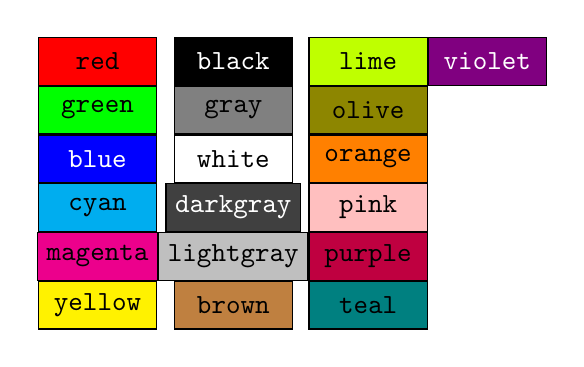
\begin{tikzpicture}[c/.style={minimum width=1.5cm,minimum height=4ex,rectangle,draw}]
  \matrix{
    \node[c,fill=red]{\verb|red|}; &&
    \node[c,fill=black,text=white]{\verb|black|}; &&
    \node[c,fill=lime]{\verb|lime|}; &&
    \node[c,fill=violet,text=white]{\verb|violet|}; \\
    \node[c,fill=green]{\verb|green|}; &&
    \node[c,fill=gray]{\verb|gray|}; &&
    \node[c,fill=olive]{\verb|olive|}; \\
    \node[c,fill=blue,text=white]{\verb|blue|}; &&
    \node[c,fill=white]{\verb|white|}; &&
    \node[c,fill=orange]{\verb|orange|}; \\
    \node[c,fill=cyan]{\verb|cyan|}; &&
    \node[c,fill=darkgray,text=white]{\verb|darkgray|}; &&
    \node[c,fill=pink]{\verb|pink|}; \\
    \node[c,fill=magenta]{\verb|magenta|}; &&
    \node[c,fill=lightgray]{\verb|lightgray|}; &&
    \node[c,fill=purple]{\verb|purple|}; \\
    \node[c,fill=yellow]{\verb|yellow|}; &&
    \node[c,fill=brown]{\verb|brown|}; &&
    \node[c,fill=teal]{\verb|teal|}; \\
  };
\end{tikzpicture}
\end{center}

\newpage
\section{\LaTeX\ tikz}
\subsection{General}
\subsubsection{Online TikZ manuel}
\url{https://tikz.dev/}\\
\subsubsection{Package and libraries}
\verb|\usepackage{tikz}| using tikz package\\
\verb|\usetikzlibrary{positioning}| Load a given tikz library\\
\subsubsection{Syntax}
\verb|\coordinate (X) at (3,5);| name a point X\\
\verb|\node[options] (X) at (3,5) {};| place a node and name it X\\

\subsection{Coordinate specifications}
\subsubsection{Coordinate calculations}
\begin{tabular}[]{p{0.1\textwidth}p{0.1\textwidth}l}
&&library needed\\
$(x,y)$&Cartesian coordinates&\\
($\theta$:r)&polar coordinates&\\
\verb |($(A)+{sin(60)}*(B)$)|         &coordinate calculations&calc\\
\verb |($(A)!.25!(B)$)|&                 partway calculations&calc\\
\verb |($(A)!3cm!(B)$)|&                 3~cm from (A) in direction of (B)&calc\\
\verb |($(A)!1.2!30:(B)$)|&              stretch by 1.2, then rotate by 30$^{\circ}$&calc\\
\verb |($(A)!(B)!(C)$)|&                 projection of point B onto line AC&calc\\
\verb |($(A)!(B)!30:(C)$)|&              project B onto line AC, then rotate by 30$^{\circ}$&calc\\
\verb '(n1-|n2)'& projection of n2 on the line passing through n1\\
\verb '(n1|-n2)'& projection of n1 on the line passing through n2\\
\verb |\node[above=1cm of| \verb|somenode.north]|&position new node 1~cm above existing anchor&positioning\\
\end{tabular}
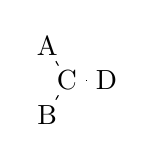
\begin{tikzpicture}
  \node (C) {C}; 
  \node (A) at ($(C)+(120:0.5)$) {A};
  \node (B) at ($(C)+(240:0.5)$) {B};
  \node (D) at ($(C)+(360:0.5)$) {D};
  \draw (C) -- (A);
  \draw (C) -- (B);
  \draw (C) -- (D);
\end{tikzpicture}
\begin{minipage}[c]{3cm}
  \begin{verbatim}
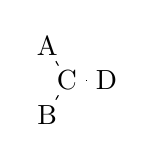
\begin{tikzpicture}
  \node (C) {C}; 
  \node (A) at ($(C)+(120:0.5)$) {A};
  \node (B) at ($(C)+(240:0.5)$) {B};
  \node (D) at ($(C)+(360:0.5)$) {D};
  \draw (C) -- (A);
  \draw (C) -- (B);
  \draw (C) -- (D);
\end{tikzpicture}
  \end{verbatim}
\end{minipage}\\
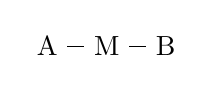
\begin{tikzpicture}
  \node (A) {A};
  \node[right=of A] (B) {B};
  \path (A) -- (B) node[midway] (M) {M};
  \draw (A) -- (M) -- (B);
\end{tikzpicture}
\begin{minipage}[c]{3cm}
  \begin{verbatim}
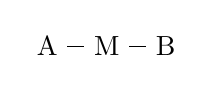
\begin{tikzpicture}
  \node (A) {A};
  \node[right=of A] (B) {B};
  \path (A) -- (B) node[midway] (M) {M};
  \draw (A) -- (M) -- (B);
\end{tikzpicture}
  \end{verbatim}
\end{minipage}\\

\textbf{Default distance between nodes}\\
\vspace{1ex}
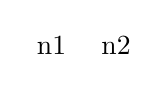
\begin{tikzpicture}[node distance=0.2cm]
  \node (n1) {n1};
  \node[right=of n1] (n2) {n2};
\end{tikzpicture}
\begin{minipage}[c]{3cm}
  \begin{verbatim}
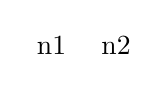
\begin{tikzpicture}[node distance=0.2cm]
  \node (n1) {n1};
  \node[right=of n1] (n2) {n2};
\end{tikzpicture}
  \end{verbatim}
\end{minipage}\\
\textbf{Shifting node positions}\\
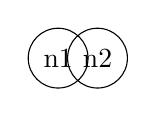
\begin{tikzpicture}
  [every node/.style={draw,circle}]
  \node(n1){n1};
  \node(n2) at ([shift={(5mm,0)}]n1) {n2};
\end{tikzpicture}
\begin{minipage}[c]{3cm}
  \begin{verbatim}
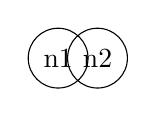
\begin{tikzpicture}
  [every node/.style={draw,circle}]
  \node(n1){n1};
  \node(n2) at ([shift={(5mm,0)}]n1) {n2};
\end{tikzpicture}
  \end{verbatim}
\end{minipage}\\

\subsubsection{Absolute positioning on the page}
\begin{verbatim}
\begin{tikzpicture}[remember picture, overlay]
  \node [] (node1) at (current page.west) {};
\end{tikzpicture}
\end{verbatim}
% 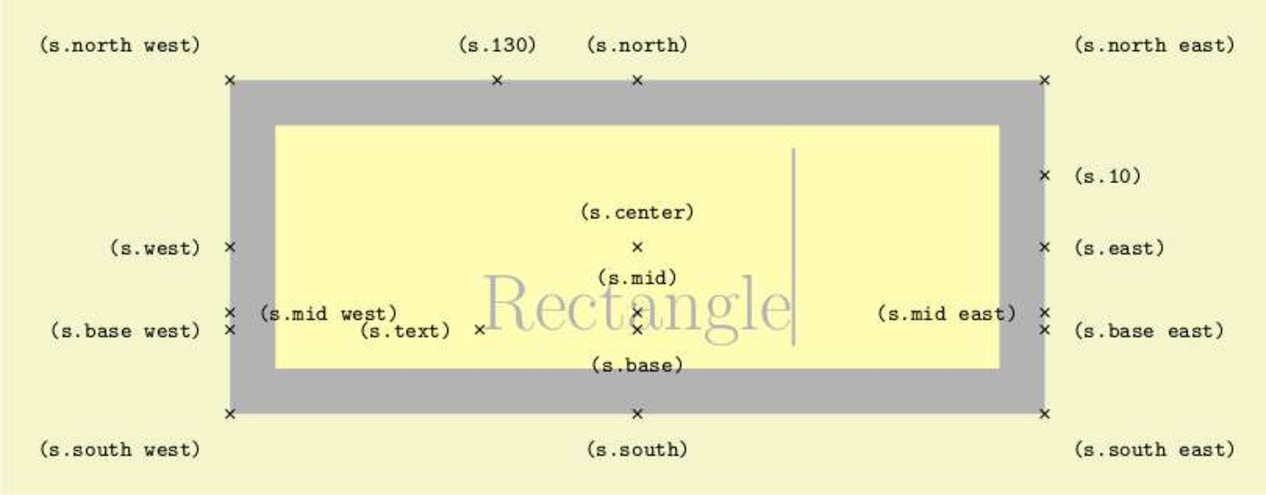
\includegraphics[width=0.33\textwidth]{figures/rectangle_shape.pdf}
\subsubsection{Matrix positioning}
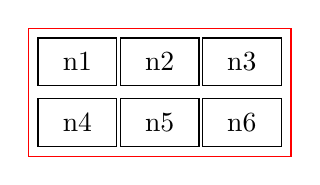
\begin{tikzpicture}
  [n/.style={draw,minimum width=1cm,minimum height=4ex,color=black}]
  \matrix[draw,color=red,column sep=0.1ex, row sep=1ex] (M) {
    \node[n] {n1}; &&
    \node[n] {n2}; &&
    \node[n] {n3}; \\
    \node[n] {n4}; &&
    \node[n] {n5}; &&
    \node[n] {n6}; \\
  };
\end{tikzpicture}
\begin{minipage}[c]{3cm}
  \begin{verbatim}
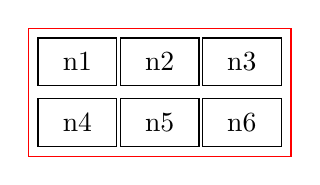
\begin{tikzpicture}
  [n/.style={draw,minimum width=1cm,
      minimum height=4ex,color=black}]
  \matrix[draw,color=red,
    column sep=0.1ex, row sep=1ex] (M) {
    \node[n] {n1}; &&
    \node[n] {n2}; &&
    \node[n] {n3}; \\
    \node[n] {n4}; &&
    \node[n] {n5}; &&
    \node[n] {n6}; \\
  };
\end{tikzpicture}
  \end{verbatim}
\end{minipage}

\subsection{Node dimension}
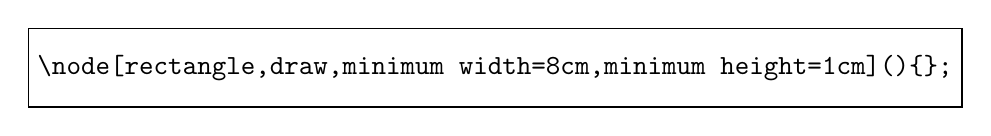
\begin{tikzpicture}
\node[rectangle,draw,minimum width=8cm, minimum height=1cm] () {\verb|\node[rectangle,draw,minimum width=8cm,minimum height=1cm](){};|};
\end{tikzpicture}

\subsection{Node shapes, filling colors and line width}
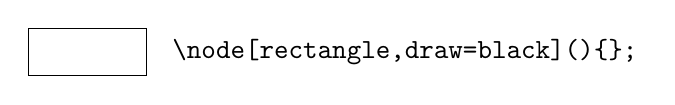
\begin{tikzpicture}
  \node[rectangle,draw=black,minimum width=1.5cm, minimum height=4ex] (rectangle) {}; 
  \node[right=0.2cm of rectangle]{\verb|\node[rectangle,draw=black](){};|};
\end{tikzpicture}
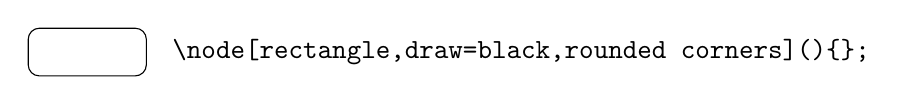
\begin{tikzpicture}
  \node[rectangle,draw=black,minimum width=1.5cm, minimum height=4ex,rounded corners] (rectangle) {}; 
  \node[right=0.2cm of rectangle]{\verb|\node[rectangle,draw=black,rounded corners](){};|};
\end{tikzpicture}
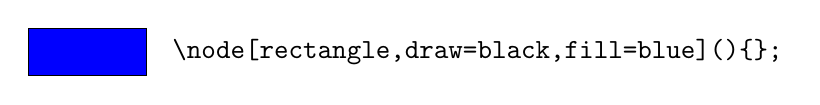
\begin{tikzpicture}
  \node[rectangle,draw=black,minimum width=1.5cm, minimum height=4ex,fill=blue] (rectangle) {}; 
  \node[right=0.2cm of rectangle]{\verb|\node[rectangle,draw=black,fill=blue](){};|};
\end{tikzpicture}
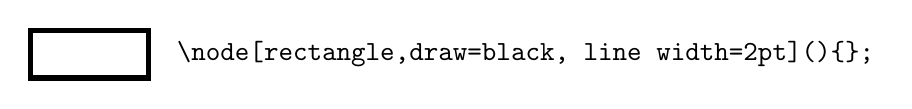
\begin{tikzpicture}
  \node[rectangle,draw=black,minimum width=1.5cm, minimum height=4ex, line width=2pt] (rectangle) {}; 
  \node[right=0.2cm of rectangle]{\verb|\node[rectangle,draw=black, line width=2pt](){};|};
\end{tikzpicture}
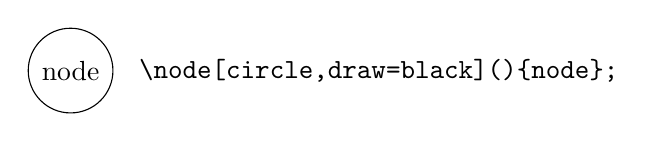
\begin{tikzpicture}
  \node[circle,draw=black] (circle) {node}; 
  \node[right=0.2cm of circle]{\verb|\node[circle,draw=black](){node};|};
\end{tikzpicture}

\subsection{Node options}
\subsubsection{Fonts and text colors}
\verb |node font=\tiny|\\
\verb |font=\bfseries| Node font in bold\\
\verb |text=blue| text color\\
\subsubsection{Text alignment in nodes}
\verb 'align=left|center|right' (handling carriage return in nodes)\\
\subsubsection{Style definition}
\verb |\begin{tikzpicture}[stylename/.style={node options...}]| Defining a node style named stylename\\
\verb |node[stylename] (node1) {};| Using a defined style\\

\vspace{1ex}
\textbf{Style definition for every node}\\
\begin{tikzpicture}[every node/.style={draw}]
  \node (n1) {n1};
  \node[right=of n1] (n2) {n2};
\end{tikzpicture}
\begin{minipage}[c]{3cm}
  \begin{verbatim}
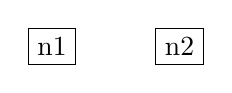
\begin{tikzpicture}[every node/.style={draw}]
  \node (n1) {n1};
  \node[right=of n1] (n2) {n2};
\end{tikzpicture}
  \end{verbatim}
\end{minipage}

\subsection{Arrows}
\begin{verbatim}
\coordinate (P1);
\coordinate[right=of P1] (P2);
\end{verbatim}
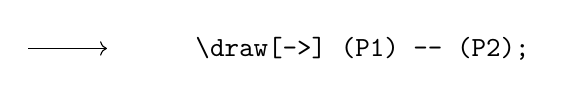
\begin{tikzpicture}
  \coordinate (P1);
  \coordinate[right=of P1] (P2);
  \draw[->] (P1) -- (P2);
  \node[right of=P2, anchor=west] {\verb|\draw[->] (P1) -- (P2);|};
\end{tikzpicture}\\
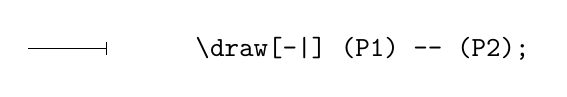
\begin{tikzpicture}
  \coordinate (P1);
  \coordinate[right=of P1] (P2);
  \draw[-|] (P1) -- (P2);
  \node[right of=P2, anchor=west] {\verb'\draw[-|] (P1) -- (P2);'};
\end{tikzpicture}
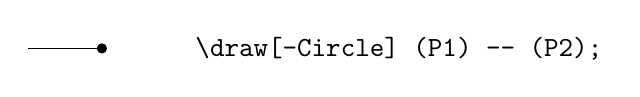
\begin{tikzpicture}
  \coordinate (P1);
  \coordinate[right=of P1] (P2);
  \draw[-Circle] (P1) -- (P2);
  \node[right of=P2, anchor=west] {\verb'\draw[-Circle] (P1) -- (P2);'};
\end{tikzpicture}
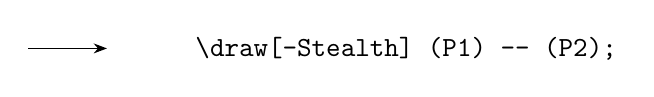
\begin{tikzpicture}
  \coordinate (P1);
  \coordinate[right=of P1] (P2);
  \draw[-Stealth] (P1) -- (P2);
  \node[right of=P2, anchor=west] {\verb|\draw[-Stealth] (P1) -- (P2);|};
\end{tikzpicture}
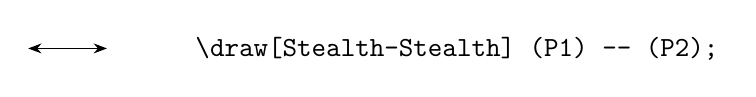
\begin{tikzpicture}
  \coordinate (P1);
  \coordinate[right=of P1] (P2);
  \draw[Stealth-Stealth] (P1) -- (P2);
  \node[right of=P2, anchor=west] {\verb|\draw[Stealth-Stealth] (P1) -- (P2);|};
\end{tikzpicture}
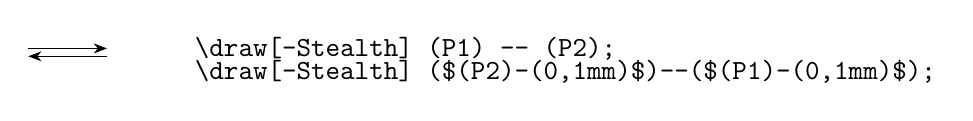
\begin{tikzpicture}
  \coordinate (P1);
  \coordinate[right=of P1] (P2);
  \draw[-Stealth] (P1) -- (P2);
  \draw[-Stealth] ($(P2)-(0,1mm)$) -- ($(P1)-(0,1mm)$);
  \node[right of=P2, anchor=west,outer sep=0] (c1) {\verb|\draw[-Stealth] (P1) -- (P2);|};
  \node[below=3mm of c1.west,outer sep=0,anchor=west] {\verb|\draw[-Stealth] ($(P2)-(0,1mm)$)--($(P1)-(0,1mm)$);|};
\end{tikzpicture}
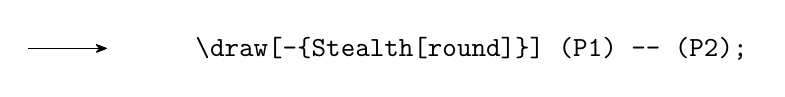
\begin{tikzpicture}
  \coordinate (P1);
  \coordinate[right=of P1] (P2);
  \draw[-{Stealth[round]}] (P1) -- (P2);
  \node[right of=P2, anchor=west] {\verb|\draw[-{Stealth[round]}] (P1) -- (P2);|};
\end{tikzpicture}
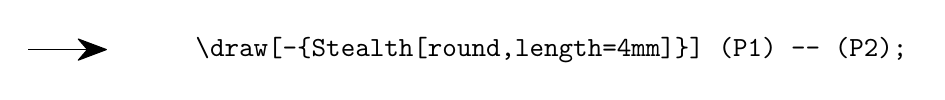
\begin{tikzpicture}
  \coordinate (P1);
  \coordinate[right=of P1] (P2);
  \draw[-{Stealth[round,length=4mm]}] (P1) -- (P2);
  \node[right of=P2, anchor=west] {\verb|\draw[-{Stealth[round,length=4mm]}] (P1) -- (P2);|};
\end{tikzpicture}
\verb |\begin{tikzpicture}[>={Stealth[round]}]| Defining an arrow style for the whole picture\\
\begin{tikzpicture}
  \coordinate (P1);
  \coordinate[right=of P1] (P2);
  \draw[-latex,line width=2pt] (P1)--(P2) node[midway,above](){a};
  \node[below=0.3cm of P1, anchor=west,xshift=-0.3cm] {\verb|\draw[-latex,line width=2pt] (P1)--(P2) node[midway,above](){a};|};
\end{tikzpicture}
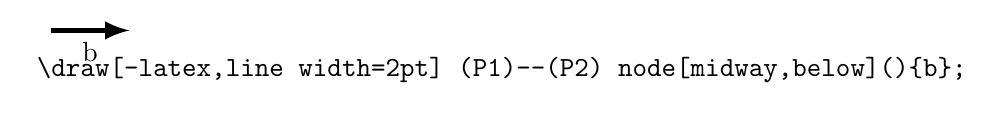
\begin{tikzpicture}
  \coordinate (P1);
  \coordinate[right=of P1] (P2);
  \draw[-latex,line width=2pt] (P1)--(P2) node[midway,below](){b};
  \node[below=0.5cm of P1, anchor=west,xshift=-0.3cm] {\verb|\draw[-latex,line width=2pt] (P1)--(P2) node[midway,below](){b};|};
\end{tikzpicture}

\subsection{Node anchors}
\begin{adjustbox}{max totalsize={0.3\textwidth}{\textheight},center}
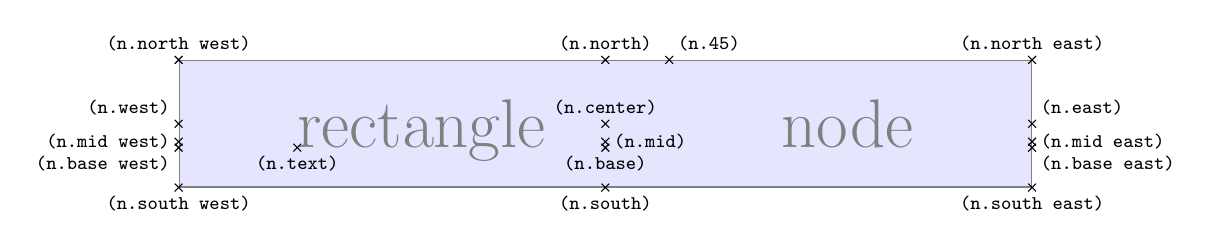
\begin{tikzpicture}[node distance = 1mm,
  shape example/.style = {
    color=black!50, draw, fill=blue!10,
    inner xsep=1.5cm, inner ysep=0.5cm,
}]
  \node[name=n,shape=rectangle,shape example]
    {\Huge rectan\smash{g}le\hspace{3cm}node};
  \foreach \anchor/\placement in
    {center/above, text/below, 45/above right,
       mid/right, mid east/right, mid west/left,
       base/below, base east/below right, base west/below left,
       north/above, south/below, east/above right, west/above left,
       north east/above, south east/below, south west/below, north west/above}
      \draw[shift=(n.\anchor)] plot[mark=x] coordinates{(0,0)}
        node[\placement,label distance = 0mm,inner sep=3pt]
          {\scriptsize\texttt{(n.\anchor)}};
\end{tikzpicture}
\end{adjustbox}
\begin{adjustbox}{max totalsize={0.3\textwidth}{\textheight},center}
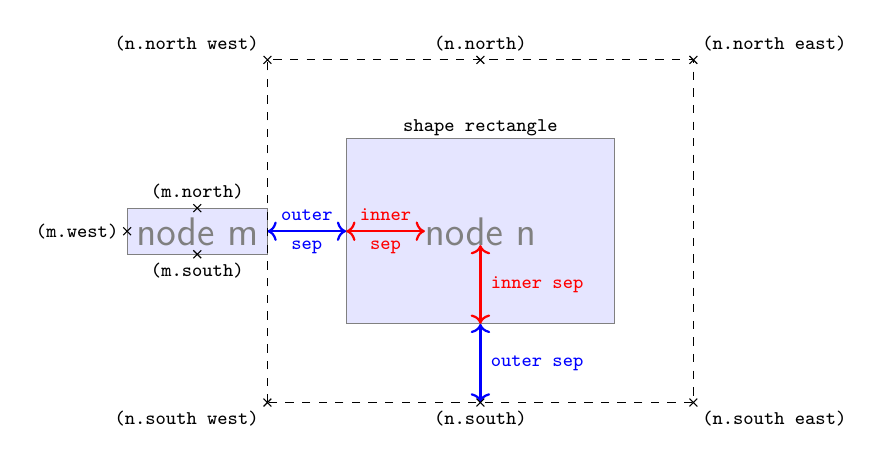
\begin{tikzpicture}[font={\scriptsize\ttfamily}]
  \node[draw,rectangle,outer sep=1cm,inner sep=1cm,color=black!50, draw, fill=blue!10]
  (n) {{\sffamily\Large node n}};
  \draw[<->,thick,blue] (n.south)
      --++(0,1cm) node[midway,right]{outer sep};
  \draw[<->,thick,red] (n.south) ++(0,1cm) 
      --++(0,1cm)node[midway,right]{inner sep};
  \node[,outer sep=0,draw,left,color=black!50, draw, fill=blue!10,] 
      (m) at(n.west) {{\sffamily\Large node m}};
  \draw[<->,blue,thick] (m.east) -- ++(1cm,0) node[midway,above] {outer}
    node[midway,below] {sep};
  \draw[<->,red,thick] ($(n.west)+(1,0)$) -- ++(1cm,0) node[midway,above] {inner}
    node[midway,below] {sep};
  \foreach \anchor/\placement in
    {south west/below left,south/below,north/above,north west/above left,
       north east/above right,south east/below right}
       \draw[shift=(n.\anchor)] plot[mark=x] coordinates{(0,0)}
        node[\placement,label distance = 0mm,inner sep=3pt] {(n.\anchor)};
  \foreach \anchor/\placement in
    {west/left,south/below,north/above}
       \draw[shift=(m.\anchor)] plot[mark=x] coordinates{(0,0)}
        node[\placement,label distance = 0mm,inner sep=3pt] {(m.\anchor)};
  \draw[dashed] (n.south west) rectangle (n.north east);
  \node[above] at ($(n.center)!0.5!(n.north)$) {shape rectangle};
\end{tikzpicture}
\end{adjustbox}
Adapted from: \url{https://tikz.org/examples/chapter-03-drawing-positioning-and-aligning-nodes}

\subsection{Geometry}
\subsubsection{Figures}
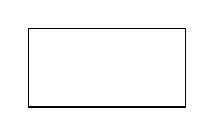
\begin{tikzpicture}
  \draw[draw=black] (0,0) rectangle ++(2,1);
\end{tikzpicture}
\begin{minipage}[c]{3cm}
  \begin{verbatim}
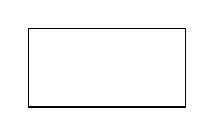
\begin{tikzpicture}
  \draw[draw=black] (0,0) rectangle ++(2,1);
\end{tikzpicture}
\end{verbatim}
\end{minipage}\\

\begin{tikzpicture}
  \path[fill=lightgray] (0,0) rectangle ++(2,1);
\end{tikzpicture}
\begin{minipage}[c]{3cm}
  \begin{verbatim}

\begin{tikzpicture}
  \path[fill=lightgray] (0,0) rectangle ++(2,1);
\end{tikzpicture}
\end{verbatim}
\end{minipage}
\subsubsection{Transformations}
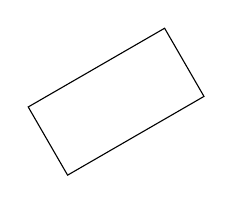
\begin{tikzpicture}
  \draw[draw,rotate=30] (0,0) rectangle ++(2,1);
\end{tikzpicture}
\begin{minipage}[c]{3cm}
  \begin{verbatim}
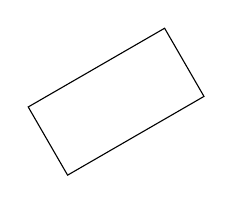
\begin{tikzpicture}
  \draw[draw,rotate=30] (0,0) rectangle ++(2,1);
\end{tikzpicture}
\end{verbatim}
\end{minipage}
\subsubsection{Shapes library}
\textbf{Callouts}\\
\verb|\usetikzlibrary{shapes.callouts}|\\
\begin{tikzpicture}
  \node[ellipse callout, draw] (hello) {Hello!};
\end{tikzpicture}
\begin{minipage}[c]{3cm}
  \begin{verbatim}
\begin{tikzpicture}
  \node[ellipse callout, draw] (hello) {Hello!};
\end{tikzpicture}
  \end{verbatim}
\end{minipage}\\
\begin{center}
\begin{tikzpicture}
  \draw [help lines] grid(3,2); 
  \node [ellipse callout,fill=red!50,callout relative pointer={(0,1)}] at (3,1) {Relative};
  \node [ellipse callout,fill=blue!50, callout absolute pointer={(0,1)}] at (1,0) {Absolute};
\end{tikzpicture}
\end{center}
\begin{verbatim}
\begin{tikzpicture}
  \draw [help lines] grid(3,2); 
  \node [ellipse callout,
   fill=red!50,
   callout relative pointer={(0,1)}] at (3,1) {Relative};
  \node [ellipse callout,
   fill=blue!50,
   callout absolute pointer={(0,1)}] at (1,0) {Absolute};
\end{tikzpicture}
\end{verbatim}

\subsection{scope environment}
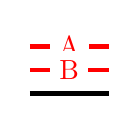
\begin{tikzpicture}[ultra thick]
  \begin{scope}[red]
    \draw (0mm,10mm) -- (10mm,10mm) 
      node[midway,fill=white] {A};
    \draw (0mm,7mm) -- (10mm,7mm)
      node[midway,fill=white] {B};
  \end{scope}
  \draw (0mm,4mm) -- (10mm,4mm);
\end{tikzpicture}
\begin{minipage}[c]{3cm}
  \begin{verbatim}
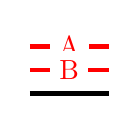
\begin{tikzpicture}[ultra thick]
  \begin{scope}[red]
    \draw (0mm,10mm) -- (10mm,10mm)
      node[midway,fill=white] {A};
    \draw (0mm,7mm) -- (10mm,7mm)
     node[midway,fill=white] {B};
  \end{scope}
  \draw (0mm,4mm) -- (10mm,4mm);
\end{tikzpicture}
  \end{verbatim}
\end{minipage}

\subsubsection{Positionning scopes relatively to other elements}
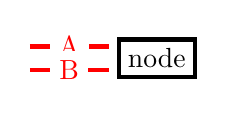
\begin{tikzpicture}[ultra thick]
  \begin{scope}[red,local bounding box=scope1]
    \draw (0mm,10mm) -- (10mm,10mm) 
      node[midway,fill=white] {A};
    \draw (0mm,7mm) -- (10mm,7mm)
      node[midway,fill=white] {B};
  \end{scope}
  \node[draw,right=0.1cm of scope1] {node};
\end{tikzpicture}
\begin{minipage}[c]{3cm}
  \begin{verbatim}
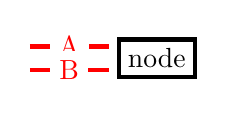
\begin{tikzpicture}[ultra thick]
  \begin{scope}[red,local bounding box=scope1]
    \draw (0mm,10mm) -- (10mm,10mm) 
      node[midway,fill=white] {A};
    \draw (0mm,7mm) -- (10mm,7mm)
      node[midway,fill=white] {B};
  \end{scope}
  \node[draw,right=0.1cm of scope1] {node};
\end{tikzpicture}
  \end{verbatim}
\end{minipage}

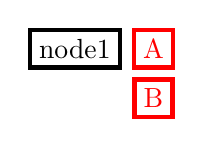
\begin{tikzpicture}[ultra thick]
  \node[draw] (node1) {node1};
  \begin{scope}[red,shift={($(node1.east)+(0.4cm,0)$)}]
    \node[draw] (A) {A};
    \node[draw,below=0.1cm of A] (B) {B};
  \end{scope}
\end{tikzpicture}
\begin{minipage}[c]{3cm}
  \begin{verbatim}
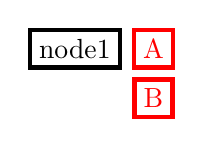
\begin{tikzpicture}[ultra thick]
  \node[draw] (node1) {node1};
  \begin{scope}[red,
          shift={($(node1.east)+(0.4cm,0)$)}]
    \node[draw] (A) {A};
    \node[draw,below=0.1cm of A] (B) {B};
  \end{scope}
\end{tikzpicture}
  \end{verbatim}
\end{minipage}

\subsection{Nested tikzpicture}
\begin{tikzpicture}[every node/.style={draw},
                    node distance=0.2cm]
  \node (n1) {n1};
  \node[right=of n1] (n2) {n2};
  \node[below=of n1] (n3) {n3};
  \node[below=of n2] (n4) {n4};
  \path (n2.east) -- (n4.east) coordinate[midway] (m);
  \node[right=of m] {
    \begin{tikzpicture}
      \node (n5) {n5}; 
      \node[right=of n5] (n6) {n6};
      \node[below=of n5] (n7) {n7};
      \node[below=of n6] (n8) {n8};
    \end{tikzpicture}
  };
\end{tikzpicture}
\begin{minipage}[c]{3cm}
  \begin{verbatim}
\begin{tikzpicture}[
    every node/.style={draw},
    node distance=0.2cm]
  \node (n1) {n1};
  \node[right=of n1] (n2) {n2};
  \node[below=of n1] (n3) {n3};
  \node[below=of n2] (n4) {n4};
  \path (n2.east) -- (n4.east)
    coordinate[midway] (m);
  \node[right=of m] {
    \begin{tikzpicture}
      \node (n5) {n5}; 
      \node[right=of n5] (n6) {n6};
      \node[below=of n5] (n7) {n7};
      \node[below=of n6] (n8) {n8};
    \end{tikzpicture}
  };
\end{tikzpicture}
  \end{verbatim}
\end{minipage}
\subsection{Variables}
\begin{tikzpicture}[node distance=1ex]
\tikzmath{
  \x1 = 3+4; \x2 = 30+40; \x3 = 300+400;
  \x4=\x1*\x2;
}
  \node(x1){x1=\x1};
  \node[below=of x1](x2){x2=\x2};
  \node[below=of x2](x3){x3=\x3};
  \node[below=of x3](x4){x4=\x4};
\end{tikzpicture}
\begin{minipage}[c]{3cm}
  \verb|\usetikzlibrary{math}|
  [\dots]
  \begin{verbatim}
\begin{tikzpicture}[node distance=1ex]
\tikzmath{
  \x1 = 3+4; \x2 = 30+40; \x3 = 300+400;
  \x4=\x1*\x2;
}
  \node(x1){x1=\x1};
  \node[below=of x1](x2){x2=\x2};
  \node[below=of x2](x3){x3=\x3};
  \node[below=of x3](x4){x4=\x4};
\end{tikzpicture}
  \end{verbatim}
\end{minipage}

\subsection{Magnifying a Part of a Picture: the spy library}
\begin{center}
\begin{tikzpicture}
  [spy using outlines={circle, magnification=4, size=2cm, connect spies}]

  \draw [help lines] (0,0) grid (3,2);

  \draw [decoration=Koch curve type 1]
    decorate { decorate{ decorate{ decorate{ (0,0) -- (2,0) }}}};

  \spy [red] on (1.6,0.3)
             in node [left] at (3.5,-1.25);

  \spy [blue, size=1cm] on (1,1)
              in node [right] at (0,-1.25);
\end{tikzpicture}
\end{center}
\begin{verbatim}
\usetikzlibrary {decorations.fractals,spy}
    [...]
\begin{tikzpicture}
  [spy using outlines={circle, magnification=4, size=2cm,
                       connect spies}]

  \draw [help lines] (0,0) grid (3,2);

  \draw [decoration=Koch curve type 1]
    decorate { decorate{ decorate{ decorate{ (0,0) -- (2,0) }}}};

  \spy [red] on (1.6,0.3)
             in node [left] at (3.5,-1.25);

  \spy [blue, size=1cm] on (1,1)
              in node [right] at (0,-1.25);
\end{tikzpicture}
\end{verbatim}

\subsection{Pics: Custom shapes}
\begin{tikzpicture}[scale=0.5]
\tikzset{
pics/mynode/.style args={#1,#2,#3}{
    code={
      \draw (0,0) -- (0.5,-0.5) -- (1,0) -- (1,1) -- (0,1) -- (0,0);
      \node[#3] (#1) at (0.5,0.5) {#2};
    }
}
}
\draw (0,0) pic{mynode={A, Hi, blue}};
\draw (0,3) pic{mynode={B, Hello, red}};
\draw (2,1.5) pic{mynode={C, Bye,}};
\draw[thick, blue] (A)--(B)--(C)--(A);
\end{tikzpicture}
\begin{minipage}[c]{3cm}
  \begin{verbatim}
\begin{tikzpicture}
\tikzset{
pics/mynode/.style args={#1,#2,#3}{
    code={
      \draw (0,0) -- (1,-1) --
        (2,0) -- (2,2) -- 
        (0,2) -- (0,0);
      \node[#3] (#1) at (1,1) {#2};
    }
}
}
\draw (0,0) pic{mynode={A, Hi, blue}};
\draw (0,3) pic{mynode={B, Hello, red}};
\draw (2,1.5) pic{mynode={C, Bye,}};
\draw[thick, blue] (A)--(B)--(C)--(A);
\end{tikzpicture}
  \end{verbatim}
\end{minipage}

\newpage
\section{Makefile}
\subsection{Variables}
\verb|$@|: target name\\
\verb|$^|: first prerequisite\\
\verb|$$X|: Access to the user var. X\\
\subsubsection{Makefile variables}
\begin{verbatim}
foo=World
all:
    echo "Hello ${foo}"
\end{verbatim}

\subsection{Syntax}
\begin{verbatim}
target: prerequisite1 prerequisite2 ...
  commands
\end{verbatim}

\subsection{User defined functions}
\begin{verbatim}
define myfunc
    echo $(1)
    echo $(2)
endef

all:
    $(call myfunc,hello world,hello the universe)
\end{verbatim}

\newpage
\section{Math}
\subsection{Running variance}
$\sigma^{2}=\frac{1}{n(n-1)}\left(n\sum_{i=1}^{n}x_{i}^2-\left(\sum_{i=1}^{n}x_i\right)^2\right)$


\newpage
\section{ImageMagick}
\subsection{Trim an image}
\begin{verbatim}
mogrify -trim <img-file> 
\end{verbatim}
\subsection{Make white color transparent}
\begin{verbatim}
mogrify -transparent white <img-file.png> 
\end{verbatim}


\end{multicols}
\end{document}
